\documentclass[preview]{standalone}

\usepackage{amsmath}
\usepackage{amssymb}
\usepackage{tikz}
\usetikzlibrary{matrix}
\usepackage{stellar}
\usepackage{definitions}

\begin{document}

\id{jordan-canonical-form}
\genpage

\section{Jordan blocks}

\begin{snippetdefinition}{jordan-block-definition}{Jordan block}
    Let \(a\in K\) and \(n\geq1\). The \emph{Jordan block of size \(n\)
    with eigenvalue \(a\)} is
    \[
        J_n(a)
        =
        \begin{pmatrix}
            a&1&0&\cdots&0\\
            0&a&1&\cdots&0\\
            0&0&a&\ddots&\vdots\\
            \vdots&\vdots&\ddots&\ddots&1\\
            0&0&\cdots&0&a
        \end{pmatrix}.
    \]
\end{snippetdefinition}

\begin{snippetproposition}{linear-primary-cyclic-module-jordan-block}{A linear primary cyclic module gives a Jordan block}
    Let \(V=K[X]v\) be a cyclic \(K[X]\)-module with \(v\neq0_V\), and
    suppose
    \[
        V\moduleisomorphic K[X]/((X-a)^n)
    \]
    for some \(a\in K\) and \(n\geq1\). Then
    \(\dim_KV=n\), and the action of \(X\), equivalently the associated
    endomorphism \(\varphi\), has matrix \(J_n(a)\) in a suitable basis.
\end{snippetproposition}

\begin{snippetproof}{linear-primary-cyclic-module-jordan-block-proof}{linear-primary-cyclic-module-jordan-block}{A linear primary cyclic module gives a Jordan block}
    The quotient has \(K\)-basis
    \[
        (X-a)^{n-1},(X-a)^{n-2},\ldots,1,
    \]
    so \(\dim_KV=n\). In \(V\), define
    \[
        w_1=(X-a)^{n-1}v,
        \quad
        w_2=(X-a)^{n-2}v,
        \quad\ldots,\quad
        w_n=v.
    \]
    These vectors form a basis. Since \((X-a)^nv=0_V\),
    \[
        Xw_1=aw_1,
    \]
    while, for \(2\leq i\leq n\),
    \[
        (X-a)w_i=w_{i-1},
        \qquad
        Xw_i=aw_i+w_{i-1}.
    \]
    These coordinate columns are exactly those of \(J_n(a)\).
\end{snippetproof}

\begin{snippetnote}{jordan-chain-from-linear-primary-module}{Jordan chains}
    The basis in the preceding proof satisfies
    \[
        (\varphi-a\identity)(w_1)=0_V,
        \qquad
        (\varphi-a\identity)(w_i)=w_{i-1}
        \quad(2\leq i\leq n).
    \]
    Thus \(w_1\) is an \eigenvector with \eigenvalue \(a\), and
    \(w_n,\ldots,w_1\) form a Jordan chain.
\end{snippetnote}

\section{Algebraically closed fields}

\begin{snippetdefinition}{algebraically-closed-field-definition}{Algebraically closed field}
    A \field \(K\) is \emph{algebraically closed} if every nonconstant
    polynomial in \(K[X]\) has a root in \(K\).
\end{snippetdefinition}

\begin{snippetproposition}{algebraically-closed-field-linear-factorization}{Characterizations of algebraic closure}
    For a \field \(K\), the following are equivalent:
    \begin{enumerate}
        \item \(K\) is algebraically closed;
        \item every nonconstant polynomial in \(K[X]\) splits into linear
        factors over \(K\);
        \item the irreducible polynomials in \(K[X]\) are precisely the
        polynomials of degree \(1\).
    \end{enumerate}
\end{snippetproposition}

\begin{snippetproof}{algebraically-closed-field-linear-factorization-proof}{algebraically-closed-field-linear-factorization}{Characterizations of algebraic closure}
    If every nonconstant polynomial has a root, then
    \(f=(X-a)g\) for some \(a\in K\). Repeating on \(g\) proves complete
    splitting by induction on degree. Complete splitting immediately
    implies the root property. It also shows that every irreducible
    polynomial has degree \(1\), and the converse follows because every
    polynomial factors into irreducibles in the
    \uniquefactorizationdomain \(K[X]\).
\end{snippetproof}

\begin{snippetexample}{algebraically-closed-field-examples}{Algebraically closed and nonclosed fields}
    The fields
    \[
        \complexnumbers
        \qquad\text{and}\qquad
        \overline{\rationalnumbers}
        =
        \{\alpha\in\complexnumbers\suchthat
        \alpha\text{ is algebraic over }\rationalnumbers\}
    \]
    are algebraically closed. The fields
    \[
        \rationalnumbers,
        \qquad
        \realnumbers,
        \qquad
        \integers/p\integers
    \]
    are not algebraically closed.
\end{snippetexample}

\begin{snippetexample}{finite-field-not-algebraically-closed-example}{An irreducible polynomial over the field with two elements}
    In \(K=\integers/2\integers\), consider
    \[
        f=X^2+X+1.
    \]
    It has no root, because
    \[
        f(0)=1\neq0,
        \qquad
        f(1)=1+1+1=1\neq0
        \quad\text{in }\integers/2\integers.
    \]
    Since \(f\) has degree \(2\), the absence of roots makes it
    irreducible. Therefore \(\integers/2\integers\) is not algebraically
    closed.
\end{snippetexample}

\section{Jordan canonical form}

\begin{snippettheorem}{jordan-canonical-form-theorem}{Jordan canonical form}
    Let \(K\) be an \algebraicallyclosedfield, let \(V\) be a
    finite-dimensional \(K\)-\vectorspace, and let
    \(\varphi\colon V\fromto V\) be a \linearendomorphism. There are
    scalars \(a_1,\ldots,a_t\in K\) and integers
    \(n_1,\ldots,n_t\geq1\) such that, in a suitable basis,
    \[
        [\varphi]
        =
        \begin{pmatrix}
            J_{n_1}(a_1)&0&\cdots&0\\
            0&J_{n_2}(a_2)&\cdots&0\\
            \vdots&\vdots&\ddots&\vdots\\
            0&0&\cdots&J_{n_t}(a_t)
        \end{pmatrix}.
    \]
    The Jordan blocks are uniquely determined up to reordering. This
    block matrix is the \emph{Jordan canonical form} of \(\varphi\).
\end{snippettheorem}

\begin{snippetproof}{jordan-canonical-form-theorem-proof}{jordan-canonical-form-theorem}{Jordan canonical form}
    Since \(K\) is algebraically closed, every monic irreducible
    polynomial in \(K[X]\) is \(X-a\) for some \(a\in K\). Hence primary
    decomposition of the associated polynomial module has the form
    \[
        V\moduleisomorphic
        \bigoplus_{i=1}^{t}K[X]/((X-a_i)^{n_i}).
    \]
    On each cyclic summand, the action of \(X\) has matrix
    \(J_{n_i}(a_i)\) in the Jordan-chain basis constructed above.
    Concatenating these bases gives the displayed form. Uniqueness is
    the uniqueness of the elementary divisors
    \((X-a_i)^{n_i}\).
\end{snippetproof}

\begin{snippetproposition}{jordan-form-characteristic-polynomial}{Characteristic polynomial in Jordan form}
    If the Jordan form of \(\varphi\) has blocks
    \(J_{n_1}(a_1),\ldots,J_{n_t}(a_t)\), then
    \[
        \chi_\varphi(X)
        =
        (X-a_1)^{n_1}\cdots(X-a_t)^{n_t}.
    \]
    Thus the \(a_i\) are the eigenvalues, repeated according to the
    sizes of their blocks.
\end{snippetproposition}

\begin{snippetproof}{jordan-form-characteristic-polynomial-proof}{jordan-form-characteristic-polynomial}{Characteristic polynomial in Jordan form}
    Each \(J_n(a)\) is triangular and has characteristic polynomial
    \((X-a)^n\). Multiply these polynomials across the block diagonal.
\end{snippetproof}

\begin{snippetcorollary}{jordan-block-diagonalizability-criterion}{Diagonalizability and Jordan blocks}
    Over an algebraically closed \field, a \linearendomorphism is
    \diagonalizable \ifandonlyif every block in its Jordan form has
    size \(1\).
\end{snippetcorollary}

\begin{snippetproof}{jordan-block-diagonalizability-criterion-proof}{jordan-block-diagonalizability-criterion}{Diagonalizability and Jordan blocks}
    If every block has size \(1\), the Jordan form is diagonal.
    Conversely, a block \(J_n(a)\) with \(n\geq2\) contributes
    algebraic multiplicity \(n\) for \(a\) but only one independent
    eigenvector. Hence the total eigenspace dimension is smaller than
    the algebraic multiplicity, so the endomorphism is not
    diagonalizable.
\end{snippetproof}

\begin{snippetexample}{same-characteristic-polynomial-distinct-jordan-forms}{The characteristic polynomial does not determine the Jordan form}
    The \(K[X]\)-modules
    \[
        K[X]/(X-a)\oplus K[X]/(X-a)
    \]
    and
    \[
        K[X]/((X-a)^2)
    \]
    are not isomorphic. They correspond respectively to
    \[
        \begin{pmatrix}a&0\\0&a\end{pmatrix}
        \qquad\text{and}\qquad
        \begin{pmatrix}a&1\\0&a\end{pmatrix}.
    \]
    Both matrices have characteristic polynomial \((X-a)^2\), but
    their Jordan-block decompositions differ, so they are not similar.
\end{snippetexample}

\section{Grouping by eigenvalue}

\begin{snippet}{jordan-blocks-grouped-by-eigenvalue}
    Suppose the distinct eigenvalues of \(\varphi\) are
    \(a_1,\ldots,a_s\). Primary decomposition can be grouped as
    \[
        V\moduleisomorphic
        \bigoplus_{i=1}^{s}
        \left(
            \bigoplus_{j=1}^{r_i}
            K[X]/((X-a_i)^{m(i)_j})
        \right),
    \]
    where
    \[
        1\leq m(i)_1\leq\cdots\leq m(i)_{r_i},
        \qquad
        \dim_KV=\sum_{i=1}^{s}\sum_{j=1}^{r_i}m(i)_j.
    \]
    For every eigenvalue \(a_i\), the corresponding Jordan blocks are
    \[
        J_{m(i)_1}(a_i),\ldots,J_{m(i)_{r_i}}(a_i).
    \]
    \[
        \begin{tikzpicture}[
            block/.style={
                draw,
                thick,
                minimum width=24mm,
                minimum height=7mm,
                align=center,
                inner sep=1pt,
                font=\scriptsize
            },
            dots/.style={
                draw,
                thick,
                minimum width=10mm,
                minimum height=7mm,
                align=center,
                inner sep=1pt,
                font=\scriptsize
            }
        ]
            \matrix[
                matrix of nodes,
                nodes in empty cells,
                row sep=3mm,
                column sep=3mm
            ] {
                |[block]| \(J_{m(1)_1}(a_1)\) & & & & & & \\
                & |[dots]| \(\cdots\) & & & & & \\
                & & |[block]| \(J_{m(1)_{r_1}}(a_1)\) & & & & \\
                & & & |[block]| \(J_{m(2)_1}(a_2)\) & & & \\
                & & & & |[dots]| \(\cdots\) & & \\
                & & & & & |[block]| \(J_{m(2)_{r_2}}(a_2)\) & \\
                & & & & & & |[dots]| \(\ddots\) \\
                & & & & & & |[block]| \(J_{m(s)_{r_s}}(a_s)\) \\
            };
        \end{tikzpicture}
    \]
\end{snippet}

\begin{snippetcorollary}{matrix-similarity-jordan-form}{Similarity and Jordan form}
    Let \(K\) be algebraically closed. Two matrices in
    \(\matrices_n(K)\) are similar \ifandonlyif they have the same
    \jordancanonicalform, up to reordering its blocks.
\end{snippetcorollary}

\begin{snippetproof}{matrix-similarity-jordan-form-proof}{matrix-similarity-jordan-form}{Similarity and Jordan form}
    This is the rational-canonical-form similarity criterion together
    with uniqueness of the Jordan blocks over an algebraically closed
    field.
\end{snippetproof}

\begin{snippetexample}{jordan-form-grouped-primary-components-example}{A Jordan form grouped by eigenvalue}
    Suppose \(a\neq b\) and
    \[
        V\moduleisomorphic
        K[X]/(X-a)
        \oplus K[X]/(X-a)
        \oplus K[X]/((X-a)^3)
        \oplus K[X]/((X-b)^2)
        \oplus K[X]/((X-b)^2).
    \]
    Then
    \[
        [\varphi]_{\mathrm J}
        =
        J_1(a)\oplus J_1(a)\oplus J_3(a)
        \oplus J_2(b)\oplus J_2(b),
    \]
    and
    \[
        \chi_\varphi=(X-a)^5(X-b)^4.
    \]
    The endomorphism is not diagonalizable because some blocks have size
    greater than \(1\).

    The original column picture records the primary components:
    \[
        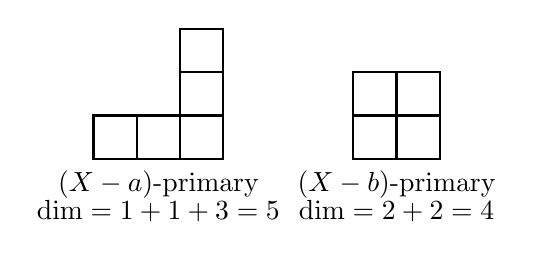
\begin{tikzpicture}[scale=0.55]
            \foreach \x/\h in {0/1,1/1,2/3} {
                \foreach \y in {1,...,\h} {
                    \draw[thick] (\x,\y-1) rectangle (\x+1,\y);
                }
            }
            \node at (1.5,-0.6) {\((X-a)\)-primary};
            \node at (1.5,-1.2) {\(\dim=1+1+3=5\)};

            \begin{scope}[xshift=6cm]
                \foreach \x/\h in {0/2,1/2} {
                    \foreach \y in {1,...,\h} {
                        \draw[thick] (\x,\y-1) rectangle (\x+1,\y);
                    }
                }
                \node at (1,-0.6) {\((X-b)\)-primary};
                \node at (1,-1.2) {\(\dim=2+2=4\)};
            \end{scope}
        \end{tikzpicture}
    \]
\end{snippetexample}

\end{document}
